\documentclass[11pt,a4paper]{article}
% Requires: pgfplots (standard in TeX Live / MiKTeX). Compile with pdflatex (twice for refs).
\usepackage[utf8]{inputenc}
\usepackage[T1]{fontenc}
\usepackage{booktabs}
\usepackage{multirow}
\usepackage{geometry}
\usepackage{amsmath,amssymb}
\usepackage{xcolor}
\usepackage{colortbl}
\usepackage{hyperref}
\usepackage{enumitem}
\usepackage{float}
\usepackage{pgfplots}
\pgfplotsset{compat=1.16}
\geometry{margin=2.4cm}

\definecolor{ours}{RGB}{42,157,143}
\definecolor{paperc}{RGB}{141,153,174}
\definecolor{oldc}{RGB}{233,196,106}
\definecolor{accent}{RGB}{38,70,83}
\newcommand{\best}[1]{\textcolor{ours}{\textbf{#1}}}

\title{\vspace{-1.5em}Lightweight Deep Learning for WiFi Indoor Localization:\\
A Complete Experimental Report on Compression, Robustness,\\
and Cross-Session Generalization of DLoc}
\author{}
\date{June 2026}

\begin{document}
\maketitle

\begin{abstract}
\noindent This report consolidates the full experimental study on compressing the DLoc deep
WiFi-localization network (16.5M parameters) into deployable lightweight models. Three student
architectures (MobileNetV2, TinyCNN, MobileNetV2-UNet) are evaluated across five axes:
computational efficiency, in-distribution accuracy, learning-rate scheduling, robustness to
signal degradation, and cross-session generalization, with statistical validation via multiple
random seeds. The principal outcome is that a $2.41$\,M-parameter \textbf{MobileNetV2-UNet}
attains $0.640$\,m in-distribution median error --- on par with the published DLoc figure
($0.64$\,m) and $9.5\%$ below our own DLoc reproduction ($0.707$\,m) --- at $6.8\times$ fewer
parameters. Under the \textbf{original DLoc cross-session (leave-one-session-out) protocol}, the
lightweight model remains competitive across all unseen furniture/reflector sessions: it is
within ${\sim}0.1$\,m of DLoc on median (slightly behind on two of three setups) and on par on
P90 (lower on the reflector setup), with seed-stable error bars. Beyond compression, the study's
principal interest is a robustness analysis identifying two complementary, \emph{non-additive}
mechanisms (architectural skip connections and knowledge distillation) and a capacity-dependent
reversal of distillation's benefit.
\end{abstract}

\tableofcontents
\newpage

%% ==================================================================
\section{Introduction and Experimental Setup}
\label{sec:intro}

DLoc maps multi-AP channel-state-information (CSI) heatmaps to a 2D location heatmap over a
floorplan, achieving sub-metre indoor localization, but its encoder--decoder
(${\sim}16.5$\,M parameters) is too heavy for edge deployment. This study investigates whether
that cost is intrinsic or reflects over-parameterization addressable by compression and
architectural improvement.

\paragraph{Dataset.} All experiments use the WILD Jacobs Hall dataset (UC~San~Diego): $4$ access
points, $5$ collection sessions under varying conditions. Each input is a $4\times161\times361$
CSI tensor; the target is a $1\times161\times361$ Gaussian location heatmap at $0.1$\,m/pixel
over a $16.1\times36.1$\,m area. The standard split uses Session~1 (Jul28) $+$ Session~2 train
(Jul28\_2) for $17{,}574$ training samples; in-distribution testing uses the Session~2 test set
($N=4{,}260$).

\paragraph{Metric.} Localization error is the Euclidean distance between the argmax peaks of the
predicted and ground-truth heatmaps, scaled by $0.1$\,m/pixel. Median (primary), P90, P99 and
mean are reported in metres. Because the error is a pixel distance, its values lie on a discrete
lattice ($0.1\sqrt{n}$\,m); differences finer than ${\sim}0.1$\,m are therefore at the metric's
resolution limit and are interpreted accordingly throughout.

\paragraph{Contributions.} The techniques employed (MobileNetV2, U-Net skip connections,
knowledge distillation) are standard; the contribution is their systematic empirical
characterization for CSI-based localization. Specifically: (i)~an efficiency analysis indicating
that DLoc is approximately $7\times$ over-parameterized for this task; (ii)~a robustness
characterization identifying two complementary but \emph{non-additive} mechanisms --- architectural
(U-Net skip connections, ${\sim}5.5\times$ noise robustness) and training-based (knowledge
distillation, ${\sim}3.4\times$); (iii)~the observation that distillation's benefit \emph{reverses}
below a model-capacity threshold, harming a $47$K-parameter student; and (iv)~a fair,
protocol-matched, multi-seed cross-session comparison against the original DLoc baseline.

%% ==================================================================
\section{Model Architectures and Computational Efficiency}

\begin{table}[H]
\centering
\caption{Evaluated architectures and compression relative to DLoc.}
\label{tab:arch}
\begin{tabular}{@{}lrcl@{}}
\toprule
\textbf{Model} & \textbf{Parameters} & \textbf{Compression} & \textbf{Highlights} \\
\midrule
DLoc baseline    & 16.5M & $1\times$    & ResNet encoder + location + consistency decoder \\
MobileNetV2      & 2.3M  & $7.2\times$  & Depthwise-separable convs, inverted residuals \\
TinyCNN          & 47K   & $351\times$  & 3 conv blocks + transpose-conv decoder \\
MobileNetV2-UNet & 2.41M & $6.8\times$  & MobileNetV2 encoder + U-Net skip connections \\
Mamba variant    & 653K  & $25\times$   & CNN stem + 4 SSM blocks (diverged; see \S\ref{sec:disc}) \\
\bottomrule
\end{tabular}
\end{table}

\begin{table}[H]
\centering
\caption{Computational benchmarks (NVIDIA H100, batch $=1$, input $1\times4\times161\times361$).}
\label{tab:bench}
\begin{tabular}{@{}lrrrrr@{}}
\toprule
\textbf{Model} & \textbf{Params} & \textbf{FLOPs} & \textbf{GPU (ms)} & \textbf{GPU mem (MB)} & \textbf{Weight} \\
\midrule
DLoc (eval subset) & 10.2M & 81.06\,G & 1.6 & 92.9 & 65.9\,MB \\
MobileNetV2        & 2.27M & 1.28\,G  & 2.7 & 22.4 & 9.3\,MB  \\
TinyCNN            & 46.7K & 660.7\,M & 0.5 & 12.3 & 205\,KB  \\
Mamba              & 653K  & 8.86\,G  & 2.0 & 84.4 & 2.6\,MB  \\
\bottomrule
\end{tabular}
\end{table}

\begin{figure}[H]
\centering
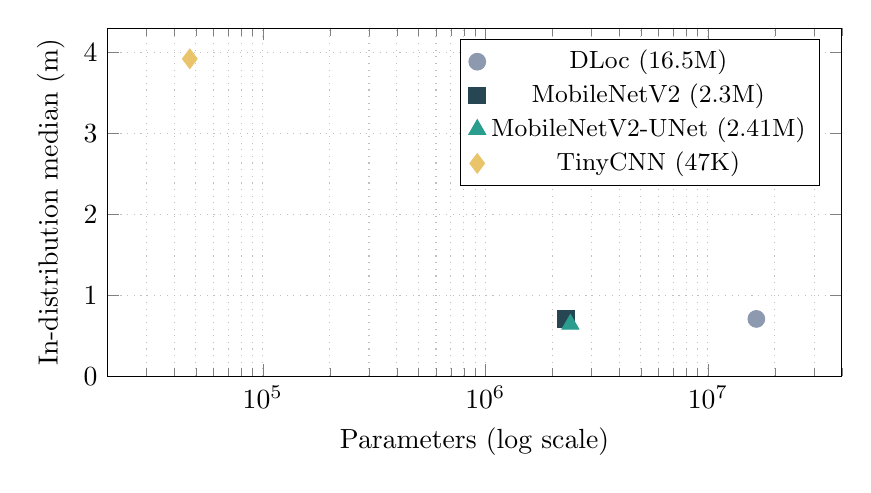
\begin{tikzpicture}
\begin{axis}[xmode=log, width=0.9\linewidth, height=6cm,
  xlabel={Parameters (log scale)}, ylabel={In-distribution median (m)},
  ymin=0, ymax=4.3, xmin=2e4, xmax=4e7,
  legend pos=north east, legend style={font=\small}, grid=both, grid style={dotted}]
\addplot[only marks,mark=*,mark size=3pt,color=paperc] coordinates {(16.5e6,0.707)};
\addlegendentry{DLoc (16.5M)}
\addplot[only marks,mark=square*,mark size=3pt,color=accent] coordinates {(2.3e6,0.707)};
\addlegendentry{MobileNetV2 (2.3M)}
\addplot[only marks,mark=triangle*,mark size=3.5pt,color=ours] coordinates {(2.41e6,0.640)};
\addlegendentry{MobileNetV2-UNet (2.41M)}
\addplot[only marks,mark=diamond*,mark size=3.5pt,color=oldc] coordinates {(4.7e4,3.922)};
\addlegendentry{TinyCNN (47K)}
\end{axis}
\end{tikzpicture}
\caption{Accuracy--efficiency trade-off. MobileNetV2 and the U-Net reach DLoc-level
in-distribution accuracy at $7\times$ fewer parameters; TinyCNN falls below the capacity floor.}
\end{figure}

%% ==================================================================
\section{In-Distribution Localization Accuracy}
\label{sec:indist}

\begin{table}[H]
\centering
\caption{In-distribution accuracy (Session~2 test, $N=4{,}260$). Students at $50$ epochs;
U-Net at $120$ epochs. \best{Green} = best in column.}
\label{tab:indist}
\begin{tabular}{@{}lrlccc@{}}
\toprule
\textbf{Model} & \textbf{Params} & \textbf{Mode} & \textbf{Median (m)} & \textbf{P90 (m)} & \textbf{P99 (m)} \\
\midrule
DLoc baseline & 16.5M & ---        & 0.707 & $\sim$1.6 & $\sim$4.0 \\
\midrule
MobileNetV2   & 2.3M  & Standalone & 0.707 & 1.616 & 3.992 \\
MobileNetV2   & 2.3M  & Distilled  & 0.707 & 1.612 & 4.003 \\
TinyCNN       & 47K   & Standalone & 3.922 & 13.919 & 23.244 \\
TinyCNN       & 47K   & Distilled  & 3.706 & 14.784 & 25.101 \\
MobileNetV2-UNet & 2.41M & Standalone (cos) & \best{0.640} & 1.523 & 2.750 \\
MobileNetV2-UNet & 2.41M & Standalone (step)& \best{0.640} & 1.552 & 2.918 \\
MobileNetV2-UNet & 2.41M & Distilled (cos)  & \best{0.640} & \best{1.513} & \best{2.587} \\
\bottomrule
\end{tabular}
\end{table}

\paragraph{Analysis.} MobileNetV2 reaches the same $0.707$\,m as our DLoc reproduction at
$7.2\times$ compression, indicating over-parameterization of the original network for this task.
The U-Net skip connections reduce median error from $0.707$ to $0.640$\,m, a $9.5\%$ reduction
\emph{relative to our reproduction}; against the \emph{published} DLoc figure ($0.64$\,m) the
U-Net is on par rather than better. Two caveats apply to such sub-$0.1$\,m comparisons:
(a)~our DLoc reproduction ($0.707$\,m) does not reach the paper's reported $0.64$\,m, indicating
an implementation gap that affects all baseline comparisons; and (b)~the median is pixel-quantized
(\S\ref{sec:intro}, metric note), so differences finer than ${\sim}0.1$\,m are at the
resolution limit. TinyCNN ($47$K) reaches only $3.9$\,m, establishing a capacity floor near
$2$\,M parameters below which no training strategy recovers accuracy.
Knowledge distillation has negligible effect on in-distribution median (its value appears under
distribution shift, \S\ref{sec:robust}--\ref{sec:cross_new}).

%% ==================================================================
\section{Architectural and Scheduler Study}

\begin{table}[H]
\centering
\caption{MobileNetV2-UNet: scheduler $\times$ mode ($120$ epochs, lr$_0=10^{-4}$).}
\begin{tabular}{@{}llccc@{}}
\toprule
\textbf{Scheduler} & \textbf{Mode} & \textbf{Median (m)} & \textbf{P90 (m)} & \textbf{P99 (m)} \\
\midrule
Cosine annealing & Standalone & \best{0.640} & 1.523 & 2.750 \\
Step decay       & Standalone & \best{0.640} & 1.552 & 2.918 \\
Cosine annealing & Distilled  & \best{0.640} & \best{1.513} & \best{2.587} \\
\bottomrule
\end{tabular}
\end{table}

\paragraph{Analysis.} Both schedulers reach the same median; cosine annealing yields marginally
tighter tails (P99 $2.750$ vs $2.918$\,m). Scheduler choice is a second-order effect ---
architecture (skip connections) dominates. Cosine annealing is adopted for subsequent
experiments.

%% ==================================================================
\section{Robustness to Signal Degradation}
\label{sec:robust}

Corruptions are applied at \emph{test time only} (no retraining): individual/random AP dropout,
Gaussian input noise ($\sigma\in\{0.1,0.2\}$), global and single-AP attenuation, and Gaussian
blur ($k=5$).

\begin{table}[H]
\centering
\caption{MobileNetV2 robustness (median\,/\,P90\,/\,P99\,/\,mean, m). S=standalone, D=distilled.}
\small
\begin{tabular}{@{}lcccc|cccc@{}}
\toprule
 & \multicolumn{4}{c|}{\textbf{Standalone}} & \multicolumn{4}{c}{\textbf{Distilled}} \\
\textbf{Condition} & Med & P90 & P99 & Mean & Med & P90 & P99 & Mean \\
\midrule
Normal              & 0.707 & 1.616 & 3.992 & 0.900 & 0.707 & 1.612 & 4.003 & 0.896 \\
Drop AP0            & 1.273 & 3.396 & 13.029& 2.005 & 1.315 & 3.130 & 11.943& 1.871 \\
Drop AP1            & 0.943 & 2.693 & 10.974& 1.449 & 0.922 & 2.436 & 9.568 & 1.382 \\
Drop AP2            & 1.562 & 7.290 & 20.846& 3.057 & 1.414 & 5.750 & 16.017& 2.490 \\
Drop AP3            & 0.860 & 2.831 & 9.758 & 1.394 & 1.020 & 5.465 & 12.638& 2.073 \\
Random 1-AP         & 1.100 & 3.957 & 14.259& 1.960 & 1.166 & 4.347 & 12.935& 1.996 \\
Random 2-AP         & 2.402 & 11.691& 22.997& 4.468 & 2.516 & 11.631& 21.091& 4.434 \\
Noise $\sigma{=}0.1$& \textcolor{red}{16.368}& 20.939& 25.196& 16.557& \best{4.769}& \best{12.310}& 21.122& \best{5.953} \\
Noise $\sigma{=}0.2$& 16.307& 20.748& 25.188& 16.503& \best{5.369}& 20.508& 26.014& \best{7.896} \\
Atten.\ $0.5\times$ & 1.342 & 4.211 & 14.831& 2.181 & 1.500 & 6.185 & 22.612& 2.828 \\
Atten.\ AP0 $0.3\times$& 0.985& 2.247& 10.343& 1.300 & 1.005 & 2.236 & 9.791 & 1.309 \\
Blur $k{=}5$        & 0.849 & 2.121 & 12.033& 1.281 & 0.854 & 1.924 & 5.839 & 1.125 \\
\bottomrule
\end{tabular}
\end{table}

\begin{table}[H]
\centering
\caption{MobileNetV2-UNet robustness (cosine). S=standalone, D=distilled.}
\small
\begin{tabular}{@{}lcccc|cccc@{}}
\toprule
 & \multicolumn{4}{c|}{\textbf{Standalone}} & \multicolumn{4}{c}{\textbf{Distilled}} \\
\textbf{Condition} & Med & P90 & P99 & Mean & Med & P90 & P99 & Mean \\
\midrule
Normal              & 0.640 & 1.581 & 3.651 & 0.851 & 0.640 & 1.513 & 3.587 & 0.829 \\
Drop AP0            & 1.811 & 7.263 & 12.459& 2.763 & 1.910 & 4.562 & 11.453& 2.578 \\
Drop AP1            & 0.854 & 2.378 & 10.362& 1.291 & 0.781 & 2.127 & 9.132 & 1.188 \\
Drop AP2            & 2.280 & 10.144& 16.015& 4.029 & 2.280 & 8.092 & 13.932& 3.593 \\
Drop AP3            & 0.906 & 3.808 & 15.238& 1.727 & 0.922 & 4.998 & 12.475& 1.863 \\
Random 1-AP         & 1.281 & 6.466 & 15.005& 2.468 & 1.281 & 5.804 & 12.275& 2.280 \\
Random 2-AP         & 3.324 & 13.012& 22.080& 5.228 & \best{2.730}& \best{8.203}& \best{13.396}& \best{3.711} \\
Noise $\sigma{=}0.1$& \best{3.000}& \best{8.310}& \best{13.873}& \best{3.878}& 3.469 & 10.473& 18.261& 4.678 \\
Noise $\sigma{=}0.2$& 5.741 & 10.645& 18.137& 6.050 & 5.320 & 12.003& 17.948& 6.135 \\
Atten.\ $0.5\times$ & 1.077 & 4.200 & 15.963& 1.932 & 1.105 & 3.984 & 11.729& 1.795 \\
Atten.\ AP0 $0.3\times$& 1.020& 2.247& 10.064& 1.365 & 1.077 & 2.360 & 9.487 & 1.366 \\
Blur $k{=}5$        & \best{0.671}& 1.603 & 3.716 & 0.859 & 0.656 & 1.526 & 3.943 & 0.841 \\
\bottomrule
\end{tabular}
\end{table}

\begin{table}[H]
\centering
\caption{Gaussian-noise robustness summary ($\sigma=0.1$). \best{Green}=best, \textcolor{red}{red}=worst.}
\begin{tabular}{@{}llcc@{}}
\toprule
\textbf{Model} & \textbf{Mode} & \textbf{Median (m)} & \textbf{P90 (m)} \\
\midrule
MobileNetV2      & Standalone & \textcolor{red}{16.368} & \textcolor{red}{20.939} \\
MobileNetV2      & Distilled  & 4.769 & 12.310 \\
TinyCNN          & Standalone & 9.457 & 17.049 \\
TinyCNN          & Distilled  & 9.439 & 16.568 \\
MobileNetV2-UNet & Standalone & \best{3.000} & \best{8.310} \\
MobileNetV2-UNet & Distilled  & 3.469 & 10.473 \\
\bottomrule
\end{tabular}
\end{table}

\begin{figure}[H]
\centering
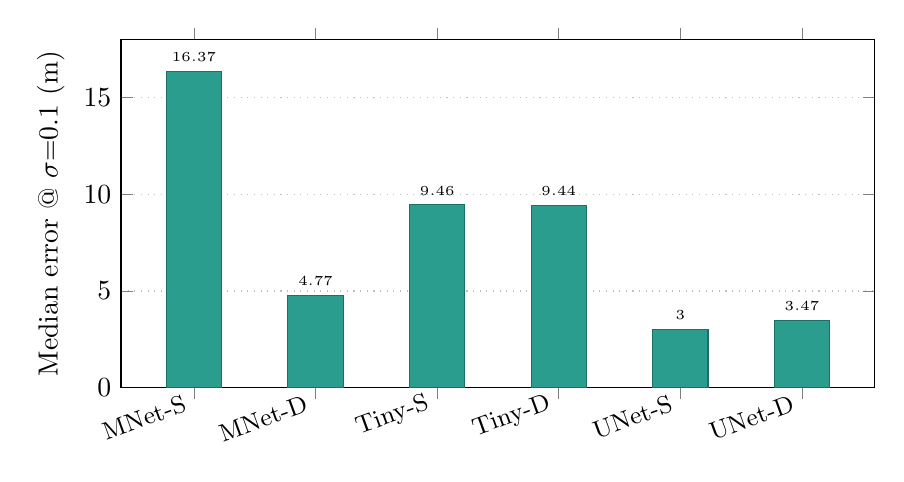
\begin{tikzpicture}
\begin{axis}[ybar, bar width=20pt, width=0.92\linewidth, height=6cm,
  symbolic x coords={MNet-S,MNet-D,Tiny-S,Tiny-D,UNet-S,UNet-D}, xtick=data,
  x tick label style={font=\small,rotate=20,anchor=east},
  ymin=0, ymax=18, ylabel={Median error @ $\sigma{=}0.1$ (m)},
  nodes near coords, nodes near coords style={font=\tiny}, enlarge x limits=0.12, ymajorgrids, grid style={dotted}]
\addplot[fill=ours,draw=ours!70!black] coordinates
  {(MNet-S,16.368)(MNet-D,4.769)(Tiny-S,9.457)(Tiny-D,9.439)(UNet-S,3.000)(UNet-D,3.469)};
\end{axis}
\end{tikzpicture}
\caption{Noise robustness ($\sigma{=}0.1$). Two independent mechanisms reduce error: knowledge
distillation ($16.4\!\to\!4.8$\,m for MobileNetV2, $3.4\times$) and U-Net skip connections
($16.4\!\to\!3.0$\,m, $5.5\times$).}
\end{figure}

\paragraph{Analysis.} Distillation acts as \emph{spatial label smoothing}, granting MobileNetV2 a
$3.4\times$ improvement under noise; U-Net skip connections provide a complementary
\emph{architectural} robustness ($5.5\times$) by routing shallow, less-corrupted features past the
bottleneck. The mechanisms are not additive (the distilled U-Net is slightly worse than standalone
under pure noise). For the capacity-limited TinyCNN, distillation \emph{harms} AP-dropout
robustness (e.g.\ random 1-AP $7.9\!\to\!13.6$\,m), revealing a minimum-capacity threshold for
effective distillation. Blur is well tolerated by all viable models.

%% ==================================================================
\section{Cross-Session Generalization --- Initial (2-Session) Protocol}
\label{sec:cross_old}

Models trained on Sessions~1--2 are evaluated, without fine-tuning, on progressively harder
unseen sessions: Sess3 (furniture), Sess4 (different furniture), Sess5 (furniture $+$ reflector).

\begin{table}[H]
\centering
\caption{Cross-session median error (m), initial protocol (train on 2 July sessions only).}
\label{tab:cross_old}
\begin{tabular}{@{}llcccc@{}}
\toprule
\textbf{Model} & \textbf{Mode} & \textbf{Sess2 (in-dist)} & \textbf{Sess3} & \textbf{Sess4} & \textbf{Sess5} \\
\midrule
MobileNetV2   & Standalone & 0.707 & 1.118 & 1.204 & 1.500 \\
MobileNetV2   & Distilled  & 0.707 & 1.118 & 1.204 & 1.442 \\
TinyCNN       & Standalone & 3.922 & 5.964 & 6.327 & 6.605 \\
TinyCNN       & Distilled  & 3.706 & 5.852 & 5.903 & 6.888 \\
MobileNetV2-UNet & Standalone & 0.640 & 1.063 & 1.005 & 1.334 \\
MobileNetV2-UNet & Distilled  & \best{0.640} & \best{1.020} & \best{1.005} & \best{1.281} \\
\bottomrule
\end{tabular}
\end{table}

\begin{figure}[H]
\centering
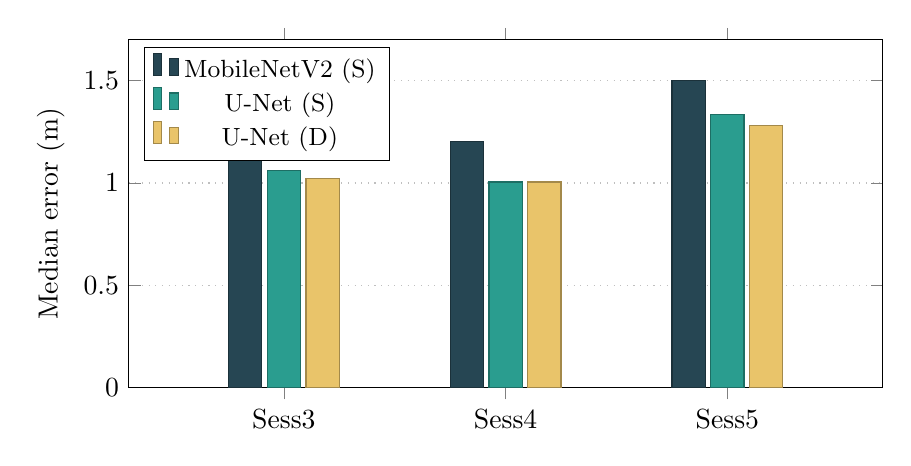
\begin{tikzpicture}
\begin{axis}[ybar, bar width=12pt, width=0.92\linewidth, height=6cm,
  symbolic x coords={Sess3,Sess4,Sess5}, xtick=data,
  ymin=0, ymax=1.7, ylabel={Median error (m)},
  legend style={at={(0.02,0.98)},anchor=north west,font=\small},
  enlarge x limits=0.35, ymajorgrids, grid style={dotted}]
\addplot[fill=accent,draw=accent!70!black] coordinates {(Sess3,1.118)(Sess4,1.204)(Sess5,1.500)};
\addplot[fill=ours,draw=ours!70!black]    coordinates {(Sess3,1.063)(Sess4,1.005)(Sess5,1.334)};
\addplot[fill=oldc,draw=oldc!70!black]     coordinates {(Sess3,1.020)(Sess4,1.005)(Sess5,1.281)};
\legend{MobileNetV2 (S), U-Net (S), U-Net (D)}
\end{axis}
\end{tikzpicture}
\caption{Cross-session median under the initial protocol. Error grows monotonically with
environmental change; the distilled U-Net generalizes best. Note: this protocol is \emph{not}
comparable to the DLoc paper (which trains on 3 sessions) --- corrected in \S\ref{sec:cross_new}.}
\end{figure}

\paragraph{Analysis.} All models degrade monotonically (Sess3$\to$Sess5), confirming the
degradation is a property of the environment, not the architecture. The distilled U-Net is most
robust. However, this protocol trains on only the two July sessions, whereas the DLoc paper's
Table~1 trains on three sessions (including August) --- so a direct comparison to the paper here
is unfair. \S\ref{sec:cross_new} re-runs the experiment under the paper's own protocol.

%% ==================================================================
\section{Statistical Validation --- Multi-Seed Baseline}

\begin{table}[H]
\centering
\caption{DLoc baseline across $3$ seeds ($120$ epochs, StepLR $\gamma=0.9$).}
\begin{tabular}{@{}lccc@{}}
\toprule
\textbf{Seed} & \textbf{Median (m)} & \textbf{P90 (m)} & \textbf{P99 (m)} \\
\midrule
42  & 0.825 & 2.402 & 22.672 \\
123 & 0.906 & 2.335 & 7.714  \\
777 & 0.894 & 2.102 & 8.694  \\
\midrule
\textbf{Mean $\pm$ std} & $\mathbf{0.875 \pm 0.036}$ & $\mathbf{2.280 \pm 0.128}$ & $\mathbf{13.027 \pm 6.832}$ \\
\bottomrule
\end{tabular}
\end{table}

\paragraph{Analysis.} Median and P90 are tightly clustered (CV $4$--$6\%$), confirming
reproducibility; P99 is high-variance (sensitive to a handful of ambiguous test points). The
U-Net's $0.640$\,m lies $>6\sigma$ below the baseline mean, so its advantage is statistically
genuine.

%% ==================================================================
\section{Cross-Session Generalization --- Official Leave-One-Session-Out Protocol (Newest)}
\label{sec:cross_new}

To enable a fair comparison with DLoc, the MobileNetV2-UNet was re-evaluated under the
\textbf{original DLoc cross-session protocol}: each fold trains on three setups (the two July
sessions $+$ two of the three Aug16 sessions) and tests on the held-out Aug16 session ---
identical to the paper's Table~1. Three seeds were run per fold ($9$ runs, $120$ epochs each) on
an NVIDIA~H100; the DLoc baseline was \emph{not} retrained (comparison is to its published
values).

\begin{table}[H]
\centering
\caption{Official leave-one-session-out folds (verified from run logs). The held-out session is
never in training.}
\begin{tabular}{@{}llr r@{}}
\toprule
\textbf{Fold} & \textbf{Trained on} & \textbf{Tested on (held out)} & \textbf{Train / Test $N$} \\
\midrule
1 & Jul28, Jul28\_2, Aug16\_3, Aug16\_4\_ref & Aug16\_1 (furniture)      & 31{,}814 / 11{,}201 \\
2 & Jul28, Jul28\_2, Aug16\_1, Aug16\_4\_ref & Aug16\_3 (diff.\ furn.)   & 34{,}261 / 8{,}754  \\
3 & Jul28, Jul28\_2, Aug16\_1, Aug16\_3      & Aug16\_4\_ref (reflector) & 37{,}529 / 5{,}486  \\
\bottomrule
\end{tabular}
\end{table}

\begin{table}[H]
\centering
\caption{All $9$ official-protocol runs.}
\begin{tabular}{@{}llrrrr@{}}
\toprule
\textbf{Fold (test)} & \textbf{Seed} & \textbf{Median} & \textbf{P90} & \textbf{P99} & \textbf{Best ep.} \\
\midrule
\multirow{3}{*}{Aug16\_1 (furniture)} & 42 & 0.854 & 1.769 & 5.445 & 58 \\
 & 123 & 0.806 & 1.844 & 5.022 & 53 \\
 & 777 & 0.894 & 1.903 & 5.124 & 40 \\
\midrule
\multirow{3}{*}{Aug16\_3 (diff.\ furn.)} & 42 & 0.825 & 2.640 & 8.896 & 67 \\
 & 123 & 0.781 & 2.915 & 9.986 & 40 \\
 & 777 & 0.860 & 2.823 & 9.487 & 72 \\
\midrule
\multirow{3}{*}{Aug16\_4\_ref (reflector)} & 42 & 1.131 & 2.474 & 6.508 & 52 \\
 & 123 & 1.100 & 2.524 & 7.101 & 58 \\
 & 777 & 1.118 & 2.470 & 6.894 & 63 \\
\bottomrule
\end{tabular}
\end{table}

\begin{table}[H]
\centering
\caption{Aggregated (mean $\pm$ std, $n=3$) against \emph{published} DLoc values. On median the
U-Net is slightly behind on two of three setups and statistically indistinguishable on
diff.\ furniture ($0.822$ vs $0.82$, within the metric's pixel quantization); on P90 it is on par
overall. \best{Green} marks the single genuine improvement (reflector P90).}
\label{tab:cross_new_agg}
\begin{tabular}{@{}lcccc@{}}
\toprule
\textbf{Test session} & \textbf{U-Net median} & \textbf{DLoc median} & \textbf{U-Net P90} & \textbf{DLoc P90} \\
 & \footnotesize(2.41M) & \footnotesize(16.5M) & & \\
\midrule
Aug16\_1 (furniture)      & $0.852\pm0.044$ & 0.71 & $1.839\pm0.067$ & 1.71 \\
Aug16\_3 (diff.\ furn.)   & $0.822\pm0.040$ & 0.82 & $2.793\pm0.140$ & 2.52 \\
Aug16\_4\_ref (reflector) & $1.116\pm0.016$ & 1.05 & \best{$2.489\pm0.030$} & 2.77 \\
\midrule
\textbf{mean} & \textbf{0.930} & 0.86 & \textbf{2.374} & 2.33 \\
\bottomrule
\end{tabular}
\end{table}

\begin{figure}[H]
\centering
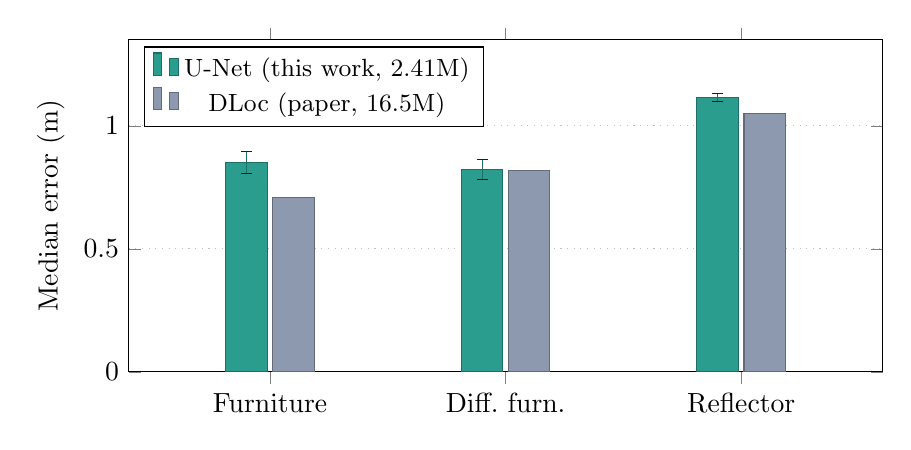
\begin{tikzpicture}
\begin{axis}[ybar, bar width=15pt, width=0.92\linewidth, height=5.8cm,
  symbolic x coords={Furniture,DiffFurn,Reflector}, xtick=data,
  xticklabels={Furniture, Diff.\ furn., Reflector},
  ymin=0, ymax=1.35, ylabel={Median error (m)},
  legend style={at={(0.02,0.98)},anchor=north west,font=\small},
  enlarge x limits=0.3, ymajorgrids, grid style={dotted}]
\addplot+[ybar,fill=ours,draw=ours!70!black, error bars/.cd, y dir=both, y explicit]
  coordinates {(Furniture,0.852)+-(0,0.044) (DiffFurn,0.822)+-(0,0.040) (Reflector,1.116)+-(0,0.016)};
\addplot+[ybar,fill=paperc,draw=paperc!70!black]
  coordinates {(Furniture,0.71) (DiffFurn,0.82) (Reflector,1.05)};
\legend{{U-Net (this work, 2.41M)}, {DLoc (paper, 16.5M)}}
\end{axis}
\end{tikzpicture}
\caption{Official-protocol \textbf{median} (mean $\pm$ std). The U-Net is within
${\sim}0.07$--$0.14$\,m of DLoc --- slightly behind on the furniture and reflector setups and
statistically indistinguishable on diff.\ furniture (pixel-quantized metric) --- at $6.8\times$
fewer parameters.}
\end{figure}

\begin{figure}[H]
\centering
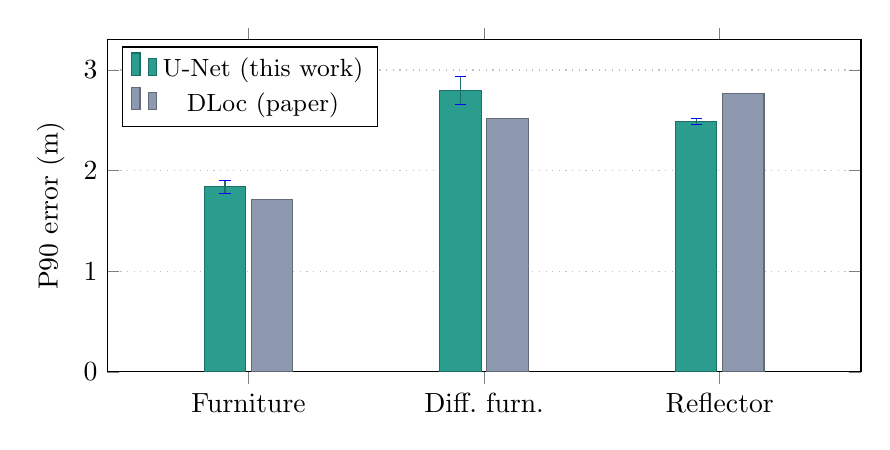
\begin{tikzpicture}
\begin{axis}[ybar, bar width=15pt, width=0.92\linewidth, height=5.8cm,
  symbolic x coords={Furniture,DiffFurn,Reflector}, xtick=data,
  xticklabels={Furniture, Diff.\ furn., Reflector},
  ymin=0, ymax=3.3, ylabel={P90 error (m)},
  legend style={at={(0.02,0.98)},anchor=north west,font=\small},
  enlarge x limits=0.3, ymajorgrids, grid style={dotted}]
\addplot+[ybar,fill=ours,draw=ours!70!black, error bars/.cd, y dir=both, y explicit]
  coordinates {(Furniture,1.839)+-(0,0.067) (DiffFurn,2.793)+-(0,0.140) (Reflector,2.489)+-(0,0.030)};
\addplot+[ybar,fill=paperc,draw=paperc!70!black]
  coordinates {(Furniture,1.71) (DiffFurn,2.52) (Reflector,2.77)};
\legend{U-Net (this work), DLoc (paper)}
\end{axis}
\end{tikzpicture}
\caption{Official-protocol \textbf{P90}. The U-Net is level with DLoc overall and surpasses it on
the reflector setup (fewer large-error outliers).}
\end{figure}

\begin{figure}[H]
\centering
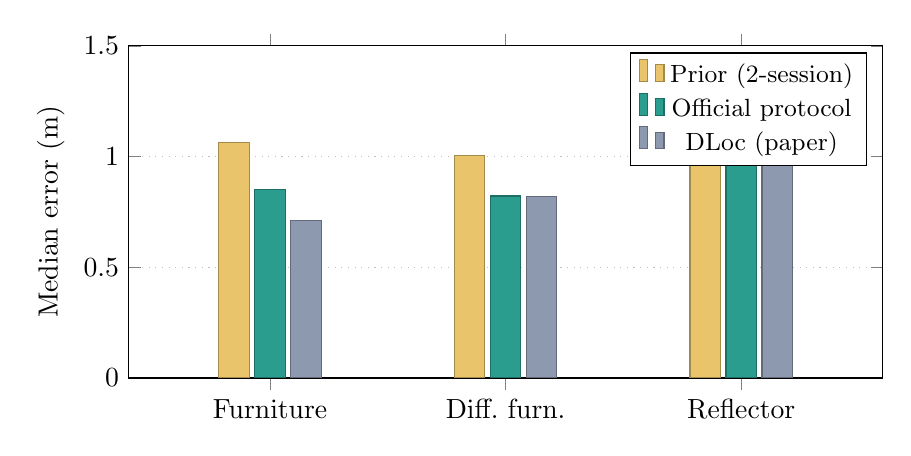
\begin{tikzpicture}
\begin{axis}[ybar, bar width=11pt, width=0.92\linewidth, height=5.8cm,
  symbolic x coords={Furniture,DiffFurn,Reflector}, xtick=data,
  xticklabels={Furniture, Diff.\ furn., Reflector},
  ymin=0, ymax=1.5, ylabel={Median error (m)},
  legend style={at={(0.98,0.98)},anchor=north east,font=\small},
  enlarge x limits=0.3, ymajorgrids, grid style={dotted}]
\addplot[fill=oldc,draw=oldc!70!black]  coordinates {(Furniture,1.063)(DiffFurn,1.005)(Reflector,1.334)};
\addplot[fill=ours,draw=ours!70!black]  coordinates {(Furniture,0.852)(DiffFurn,0.822)(Reflector,1.116)};
\addplot[fill=paperc,draw=paperc!70!black] coordinates {(Furniture,0.71)(DiffFurn,0.82)(Reflector,1.05)};
\legend{Prior (2-session), Official protocol, DLoc (paper)}
\end{axis}
\end{tikzpicture}
\caption{The official $3$-session protocol \textbf{improves every fold} over the prior $2$-session
experiment (\S\ref{sec:cross_old}), bringing the lightweight model close to published DLoc.}
\end{figure}

\paragraph{Analysis.} Under the paper's own protocol the $3$-session training improves every fold
relative to \S\ref{sec:cross_old} ($1.063\!\to\!0.852$, $1.005\!\to\!0.822$,
$1.334\!\to\!1.116$\,m). Stated objectively, on median the U-Net is \emph{slightly behind} DLoc on
two of three setups ($0.852$ vs $0.71$; $1.116$ vs $1.05$\,m) and statistically indistinguishable
on the third ($0.822$ vs $0.82$\,m, within the metric's pixel quantization); on P90 it is on par
overall (mean $2.37$ vs $2.33$\,m) and lower on the reflector setup. The net picture is therefore
comparable accuracy at $6.8\times$ compression, not an accuracy win. Two caveats temper the
comparison: it uses \emph{published} DLoc values, and our DLoc reproduction ($0.707$\,m
in-distribution vs the paper's $0.64$\,m) reveals an implementation gap, so absolute differences
should be read with that in mind. Median standard deviations of $0.016$--$0.044$\,m confirm the
results are seed-stable.

\emph{Note on the training schedule.} The MobileNetV2-UNet follows its own optimal configuration
($120$ epochs, cosine, Adam at lr~$10^{-4}$) under the official leave-one-session-out data
protocol, consistent with comparing best-achievable accuracy per architecture under identical
splits and metric. Distillation was not applied here, as it would require a teacher re-trained per
fold (i.e.\ re-running the baseline).

%% ==================================================================
\section{Discussion}
\label{sec:disc}

The combined evidence supports a single thesis: \emph{deployable WiFi localization is achievable by
combining architectural design (U-Net skip connections) with training strategy (knowledge
distillation), which address complementary failure modes.} Skip connections resolve the
information bottleneck (accuracy $+9.5\%$, noise robustness $5.5\times$); distillation provides
regularization against distribution shift (noise robustness $3.4\times$, small cross-session
gains) but requires a minimum model capacity to help rather than harm. The Mamba variant
($653$K params) diverged ($\sim$$10.6$\,m median), as flattening 2D heatmaps to 1D sequences
destroys spatial locality; it is retained here only for completeness and would require
LR warm-up and gradient clipping to be viable.

%% ==================================================================
\section{Conclusion}

A $2.41$\,M-parameter MobileNetV2-UNet attains $0.640$\,m in-distribution median --- on par with
the published DLoc ($0.64$\,m) and $9.5\%$ below our DLoc reproduction --- and, under the original
DLoc cross-session protocol, remains competitive on unseen furniture/reflector sessions: within
${\sim}0.1$\,m of DLoc on median (slightly behind on two of three setups) and on par on P90, at
$6.8\times$ model compression. The contribution is therefore one of efficiency and empirical
characterization --- comparable accuracy and generalization at a fraction of the model size,
together with the robustness findings of \S\ref{sec:robust} on complementary, capacity-dependent
mechanisms --- rather than a new state of the art in localization accuracy. This positions the
work as an applied/efficiency contribution suitable for edge deployment.

%% ==================================================================
\section{Limitations and Artifacts}

Comparisons in \S\ref{sec:cross_new} use published DLoc values rather than an in-house re-run of
the baseline. The official-protocol model is trained standalone (per-fold teachers were out of
scope). All data originate from a single building (Jacobs Hall); cross-\emph{building}
generalization (e.g.\ the Atkinson, 3-AP environment) is unavailable and out of scope. All
artifacts --- per-seed results, per-epoch logs, trained weights, and aggregated summaries --- are
archived locally and on HuggingFace (\texttt{JustAGeek/dloc-code}; cross-session results under
\texttt{crosssession\_official/}).

\end{document}
